\documentclass[11pt]{article}
\usepackage{graphicx}
\usepackage{tcolorbox}
\usepackage{amsmath}
\usepackage{multicol}
\usepackage{amssymb}
\usepackage{amsthm}
\usepackage{amsfonts}
\usepackage{float}
\usepackage[font=small,skip=0pt]{caption}
\makeatletter
\captionsetup[figure]{skip=0pt}
\title{\vspace{-5.0cm}KTH Royal Institute of Technology\\ DD2424-VT19-1 Deep Learning in Data Science\\ Assignment 1 Bonus Points }
\author{Marina Herrera Sarrias }
\begin{document}
\maketitle

\section{Exercise 2.1} 
\begin{tcolorbox}
Reports on your trained network with the best test accuracy, what improvements you made and which ones brought the largest gains.
\end{tcolorbox}

The optimization performed on the network consisted on:\\
\begin{itemize} 
	\item Shuffle the order of the training examples at the beginning of each epoch.
	\item Decaying the learning rate by a factor of $2$ after every $5$ epochs. 
	\item A grid search for finding \textit{good} values of the hyper-parameters: \texttt{eta}, \texttt{lambda}, \texttt{n\_batch}, and \texttt{n\_epoch}. I tested all possible combination of all the following parameter values:
	\begin{itemize}
		\item \texttt{eta} = [$1\text{e-}4$, $1\text{e-}3$, $1\text{e-}2$]
		\item \texttt{lambda} = [$1\text{e-}5$, $1\text{e-}4$, $1\text{e-}3$, $1\text{e-}2$, $1\text{e-}1$, $0$]
		\item \texttt{n\_batch and n\_epochs}= $[(10, 200), (50, 200)]$
	\end{itemize}
	\item The grid search was also applied to the  ordering shuffle and the decaying learning rate cases. \\

From all the cases above mentioned the parameter setting that maximized the accuracy of the model was under the data shuffling scenario, with a $39.07\%$ of the test accuracy, using the following parameters:  \texttt{eta} = $0.001$, \texttt{lambda} = $0.01$, \texttt{n\_batch and n\_epochs}= $[(10, 200)]$. Which compared to the test accuracy results obtained using the original model, under the same parameter setting, there is a $0.81\%$ improvement.\\

This, as the first epochs are usually the ones that bring more gain, and when no shuffling is performed, the same data will always be at the beginning of the training.\\

The second best model was obtained applying \texttt{eta} decay, with a test accuracy of $38.87\%$ for the parameter setting: \texttt{eta} = $0.001$, \texttt{lambda} = $0.0001$, \texttt{n\_batch and n\_epochs}= $[(50, 200)]$, which has only show a small $(0.26\%)$ improvement with respect to the non-optimized model, using the same parameter setting.\\ 

In general, the results obtained after applying the different optimization tricks did not result in big improvements. Most of the results obtained for the different parameter settings were very similar, among the three scenarios. 
\end{itemize}

\section{Exercise 2.2} 
\begin{tcolorbox}
Compare the test accuracy of the network trained with the SVM loss compared to the cross-entropy loss (for several sensible training parameter settings).
\end{tcolorbox}

After applying the same grid search proposed in the previous section the test accuracy obtained with the Network trained using the cross-entropy loss had the highest values most of the time ($30/36$)  in comparison with  the ones obtained on the Network trained with the SVM multi-class loss($6/36$).\\

This, in addition to the fact that training the Network using the SVM multi-class, was considerably more computationally expensive, compared to the Network trained using cross-entropy loss.\\

Some of the tested parameter settings:
 \pagebreak
\begin{itemize}
	\item {\texttt{lambda=0.1, n\_epochs=200, n\_batch=10, eta=.01}}

\begin{figure}[H]
	\centerline{\includegraphics[width=195mm,scale=0.7]{svm1.png}}
	\caption{ The network was trained with the following parameter settings$:$ \texttt{n\_batch}$=200$ \texttt{eta}$=0.01$, \texttt{n\_epochs}$=10$ and  \texttt{lambda}$=0.1$. Using the SVM multi-class loss function}
	\label{fig:1.1}
\end{figure}

\begin{figure}[H]
	\centerline{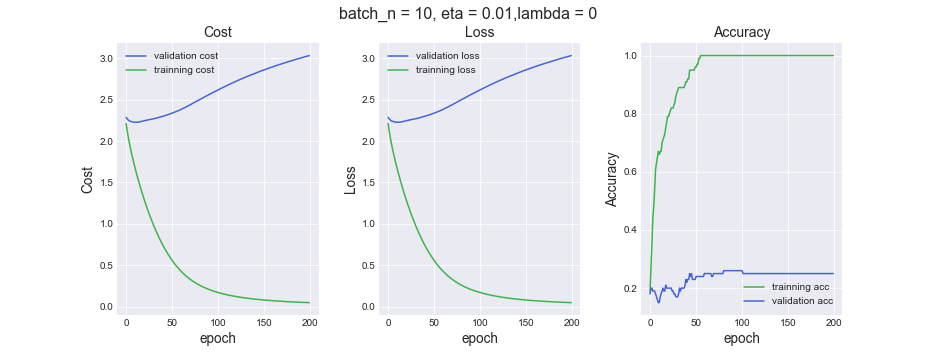
\includegraphics[width=195mm,scale=0.7]{test1.png}}
	\caption{ The network was trained with the following parameter settings$:$ \texttt{n\_batch}$=200$ \texttt{eta}$=0.01$, \texttt{n\_epochs}$=10$ and  \texttt{lambda}$=0.1$ Using the cross-entropy loss.}
	\label{fig:1.2}
\end{figure}
 \pagebreak
\item {\texttt{lambda=$1\text{e-}5$, n\_epochs=200, n\_batch=50, eta=.001}}

\begin{figure}[H]
	\centerline{\includegraphics[width=195mm,scale=0.7]{svm3.png}}
	\caption{ The network was trained with the following parameter settings$:$ \texttt{n\_batch}$=200$ \texttt{eta}$=0.01$, \texttt{n\_epochs}$=10$ and  \texttt{lambda}$=0.1$. Using the SVM multi-class loss function}
	\label{fig:1.1}
\end{figure}

\begin{figure}[H]
	\centerline{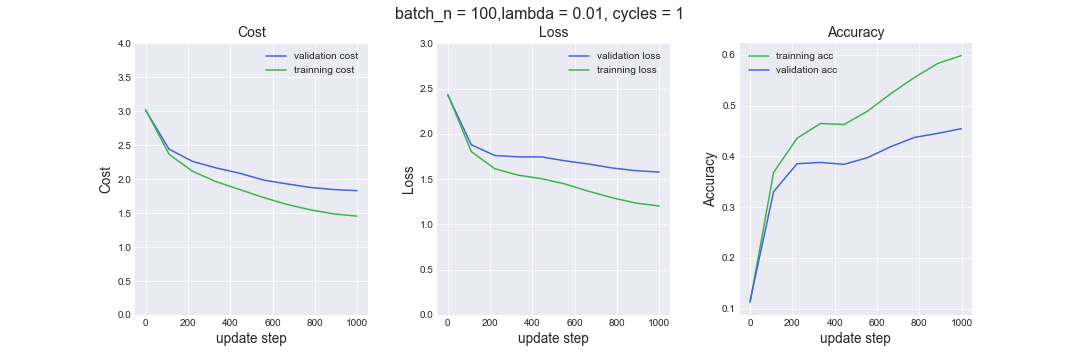
\includegraphics[width=195mm,scale=0.7]{test2.png}}
	\caption{ The network was trained with the following parameter settings$:$ \texttt{n\_batch}$=200$ \texttt{eta}$=0.01$, \texttt{n\_epochs}$=10$ and  \texttt{lambda}$=0.1$ Using the cross-entropy loss.}
	\label{fig:1.6}
\end{figure}
 \pagebreak
\item {\texttt{lambda=0.001, n\_epochs=200, n\_batch=50, eta=0.0001}}

\begin{figure}[H]
	\centerline{\includegraphics[width=195mm,scale=0.7]{svm4.png}}
	\caption{ The network was trained with the following parameter settings$:$ \texttt{n\_batch}$=200$ \texttt{eta}$=0.0001$, \texttt{n\_epochs}$=50$ and  \texttt{lambda}$=0.001$. Using the SVM multi-class loss function}
	\label{fig:1.1}
\end{figure}

\begin{figure}[H]
	\centerline{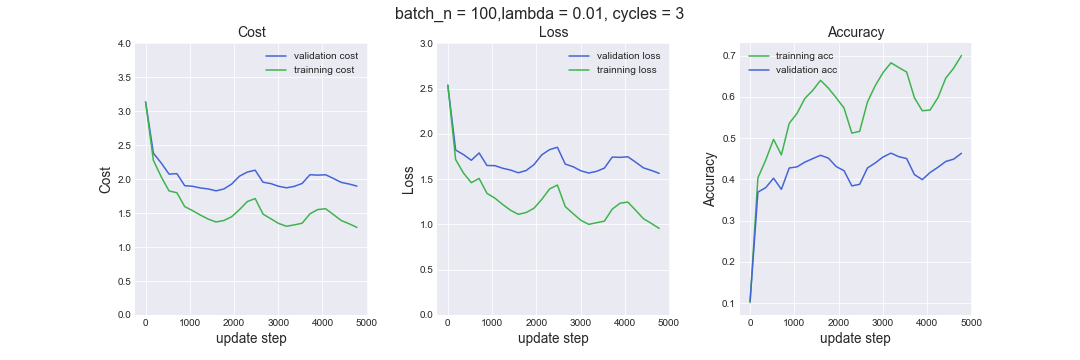
\includegraphics[width=195mm,scale=0.7]{test3.png}}
	\caption{ The network was trained with the following parameter settings$:$ \texttt{n\_batch}$=200$ \texttt{eta}$=0.0001$, \texttt{n\_epochs}$=50$ and  \texttt{lambda}$=0.001$ Using the cross-entropy loss.}
	\label{fig:1.4}
\end{figure}


\end{itemize}




\end{document}
